\chapter{Porting the Modular Run-Time}

The modular run-time has been designed specifically with portability in mind. All of OS-related functions are grouped together in one file, be it the inline functions, or the function pointers.

The run-time comes with a \verb=posix.c= file which is a sample file that shows how to hook up all possible function pointers to the run-time and allows the run-time to work on most Unix-based operating systems, including OS X and Linux.

To demonstrate the easiness of porting the run-time to even obscure platforms, the run-time has been successfully ported to 2 operating systems one may consider obscure.

\section{Windows 3.11}

Windows 3.11 is a 16-bit operating system, developed by Microsoft and released in 1993, almost 20 years ago. Notice that the Modular Run-time has been successfully run on a 16-bit, 32-bit and a 64-bit operating system without changing a single line other than the OS-specific function pointers!

As finding a real computer running such an OS would be nearly impossible, so it is run in a DOSBox emulator. Borland Turbo C++ 4.5 has been installed and the run-time, including the testing main function has been compiled.

Surprisingly enough, the Turbo C++ supplies basic C libraries with \verb=malloc= and others, so actually the \verb=posix.c= file could be used. It might sound that it went very smoothly with no effort, however, there were a few hiccups, that were not caused by error in design, but technical limitations of the platform. Other than that, the process of getting the run-time run on Windows 3.11 was a matter of a few minutes.

\begin{itemize}
  \item{\bf{File name length}} Due to limitations of FAT-16, all filenames must have 8 or less characters, plus the extension, otherwise they get truncated to 6 characters and the infamous tilde-number suffix. This would not be a big problem cosmetically, however, the compiler could not find includes of files that had longer names. Hence many files needed to be renamed.
  \item{\bf{C89}} Many C features that are nowadays considered for granted, such as \verb=//= comments, declaring variables whenever it fits, not just at the beginning of a scope, inlining functions, etc., were not available at that time. Hence it has been made sure for all run-time code to be compilable with the C89 standard.
  \item{\bf{No pthread}} As there is not much documentation for Windows 3.11 anymore, mostly due to the fact that back in the day most documentation was printed, not online or distributed in any digital form, it cannot be said for sure that Windows 3.11 did not have threading support, but all RW locking had to be thrown away and no-op'ed. 
\end{itemize}

\begin{figure}[H]
  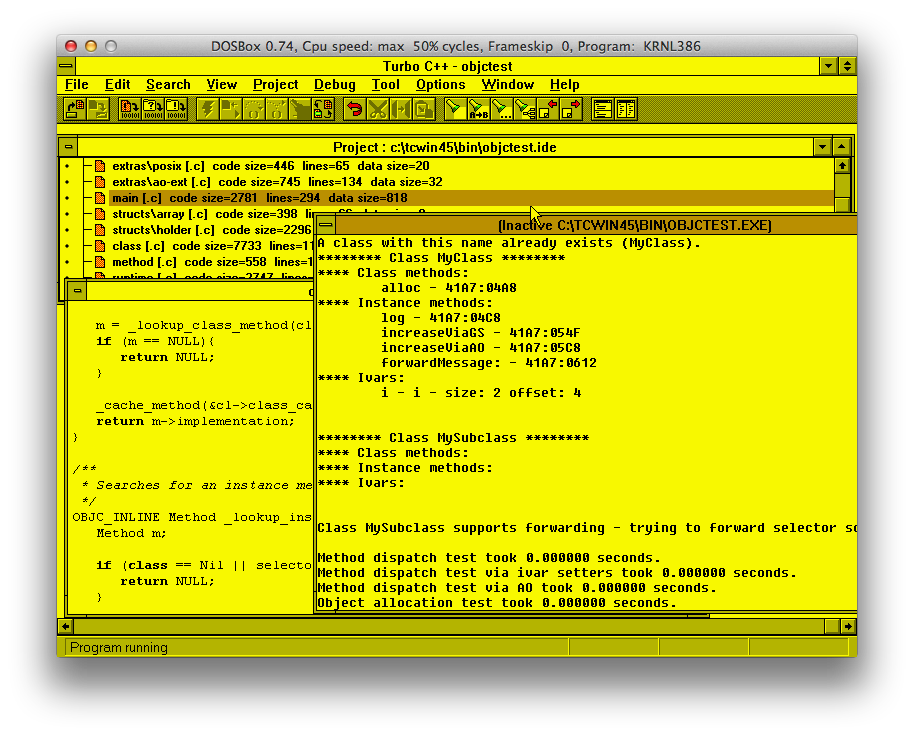
\includegraphics[width=\textwidth]{img/dos_box_3_11.png}
  
  \centering{}
  \caption{The modular run-time running on Windows 3.11 in a DOSBox emulator.}
  \label{fig:win_3_11}
\end{figure}

\section{Kalisto HeSiVa}

During a course on Operating Systems, the students are divided into teams of 3 and get to build up a very bare kernel called \emph{Kalisto} (that has a very simple loader, threading and a memory allocator) into an operating system with virtual memory, user space, allowing users to install and launch their own programs. And all this were to run in a 32-bit MIPS simulator.

When designing some tests for the modular run-time, this ``operating system" has come to mind as the ultimate challenge.

Interestingly, it took less work than porting it to Windows 3.11. The \verb=posix.c= file has been left out and it took only 32 lines of code (including some white space) to get the run-time running on such an operating system. The lines of code that were inserted can be seen in figure ~\ref{fig:hesiva_code}.

\begin{figure}[H]
  \begin{verbatim}
  static void *_zero_alloc(unsigned long size){
    void *memory = malloc(size);
    objc_memory_zero(memory, size);
    return memory;
  }
  
  static void _abort(const char *msg){
    printf(msg);
    kill(process_self());
  }
  
  static objc_rw_lock _rw_lock_creator(void){
    mutex_t *m = malloc(sizeof(mutex_t));
    mutex_init(m);
    return (objc_rw_lock)m;
  }
  
  static void _rw_lock_destroyer(objc_rw_lock lock){
    mutex_destroy((mutex_t*)lock);
    free(lock);
  }
  
  static void init_kalisto(void){
    objc_runtime_set_allocator(malloc);
    objc_runtime_set_deallocator(free);
    objc_runtime_set_zero_allocator(_zero_alloc);
    objc_runtime_set_abort(_abort);
    objc_runtime_set_log(printf);
    objc_runtime_set_rw_lock_creator(_rw_lock_creator);
    objc_runtime_set_rw_lock_destroyer(_rw_lock_destroyer);
    objc_runtime_set_rw_lock_rlock(mutex_lock);
    objc_runtime_set_rw_lock_wlock(mutex_lock);
    objc_runtime_set_rw_lock_unlock(mutex_unlock);
  }
  \end{verbatim}
  \centering{}
  \caption{The only lines that needed to be added in order for the run-time to run on kalisto HeSiVa.}
  \label{fig:hesiva_code}
\end{figure}

\begin{figure}[H]
  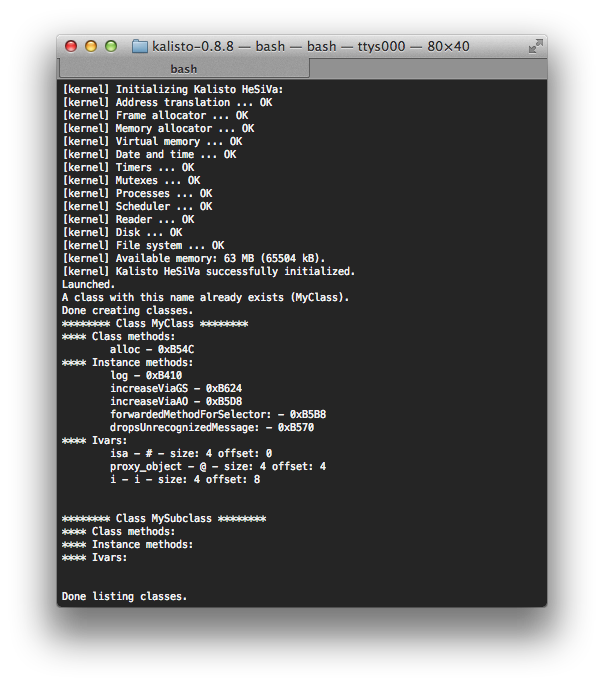
\includegraphics[width=\textwidth]{img/hesiva.png}
  
  \centering{}
  \caption{The modular run-time running on kalisto HeSiVa.}
  \label{fig:hesiva_run}
\end{figure}
